\documentclass[a4paper]{scrreprt}
\usepackage[left=4cm,bottom=3cm,top=3cm,right=4cm,nohead,nofoot]{geometry}
\usepackage{import,graphicx,tabularx,listings,enumitem,subcaption}
\usepackage{xparse,multirow}
\usepackage{xcolor}
\usepackage{float}
\usepackage{listings}
\usepackage[utf8]{inputenc}
\lstset{
    language=Python,
    basicstyle=\ttfamily\small,
    keywordstyle=\color{blue},
    stringstyle=\color{orange},
    commentstyle=\color{gray},
    showstringspaces=false,
    frame=single,
    breaklines=true,
    tabsize=4,
    captionpos=b
}

\setlength{\textfloatsep}{16pt}
\renewcommand{\labelenumi}{\alph{enumi})}
\renewcommand{\labelenumii}{\arabic{enumii}) }

% Base info for header
\newcommand{\baseinfo}[5]{
  \begin{center}
    \begin{tabular}{p{15cm}r}
      \vspace{-4.5pt}{ \Large \bfseries #1} & \multirow{2}{*}{} \\[0.4cm]
      #2 & \\[0.5cm]
    \end{tabular}
  \end{center}
  \vspace{-18pt}\hrule\vspace{6pt}
  \begin{tabular}{ll}
    \textbf{Names:} & #4\\
    \textbf{Group:} & #5\\
  \end{tabular}
  \vspace{4pt}\hrule\vspace{2pt}
  \footnotesize \textbf{Software Testing} \hfil - \hfil Summer 2024 \hfil - \hfil #3 \hfil - \hfil Sibylle Schupp / Daniel Rashedi \hfil \\
}

\lstdefinestyle{pythongrey}{
    language=Python,
    basicstyle=\ttfamily\small,
    keywordstyle=\color{blue},
    commentstyle=\color{gray},
    stringstyle=\color{green!50!black},
    backgroundcolor=\color{gray!10},
    showstringspaces=false,
    breaklines=true,
    frame=single,
    framesep=3pt,
    tabsize=4,
    numbers=left,
    numberstyle=\tiny\color{gray},
    numbersep=8pt,
    captionpos=b
}

% Question and answer environments
\newcounter{question}
\NewDocumentEnvironment{question}{m o}{%
  \addtocounter{question}{1}%
  \paragraph{\textcolor{red}{Task~\arabic{question}} - #1\hfill\IfNoValueTF{#2}{}{[#2]}}
  \leavevmode\\%
}{%
  \vskip 1em%
}

\NewDocumentEnvironment{aiTask}{}{
  \paragraph{\textcolor{red}{AI Review Task}}
  \leavevmode\\
}{
  \vskip 1em
}

\NewDocumentEnvironment{answer}{}{%
  \vspace{6pt}
  \leavevmode\\
  \textit{Answer:}\\[-0.25cm]
  {\color{red}\rule{\textwidth}{0.4mm}}
}{%
  \leavevmode\\
  {\color{red}\rule{\textwidth}{0.4mm}}
}

% ======= STUDENTS: START EDITING BELOW THIS LINE =======
\newcommand{\projectinfo}[4]{\baseinfo{Project - Submission Sheet}{#1}{#2}{#3}{#4}}
\newcommand{\name}{[Maxim Zilke, Yossef Al Buni]}
\newcommand{\group}{[2]}

\begin{document}
\projectinfo{Software Testing - Random Testing\small}{\today}{\name}{\group}


%%%%%%%%%%%%%%%%
%%% Phase 01 %%%
%%%%%%%%%%%%%%%%
%%%%%%%%%%%%%%%%%%%%%%%%%%%%%%%%%%%%%%%%%%%%%%%%%%%%%%%%%%%%%%
\begin{question}{Random Testing}
  \begin{enumerate}[topsep=0pt, leftmargin=*]
    \item Add the 4 generated Python tests of each group member to your repository in the corresponding folder. Add a README.md file that explains how to build / run the tests.
    %%%%%%%%%%%%%%%%%%%%%%%%%%%%%%%%%%%%%%%%%%%%%%%%%%%%%%%%%%%%%%
Maxim Zilka
                \begin{lstlisting}[caption={Hypothesis-Test für \_normalize\_key}, label={lst:normalize-key}]

from hypothesis import given
from hypothesis.strategies import floats, lists, integers, text
from hypothesis.strategies import just
import re
import string
import pytest
from hypothesis.strategies import text
import sys
from streamlink.options import Options



@given(
    prefix=text(alphabet=string.ascii_lowercase + "_-"),
    suffix=text(alphabet=string.ascii_lowercase + "_-")
)
def test_normalize_key_contains_dash(prefix, suffix):
    input_str = prefix + "_" + suffix  # manuelle eingabe von "_", um in jedem test sicherzustellen, dass ein "_" vorhanden ist
    print(f"Generated input for prefix: {prefix}")  # Eingabe anzeigen
    print(f"Generated input for suffix: {suffix}")  # Eingabe anzeigen
    result = Options._normalize_key(input_str)

    # Es darf kein "_" vorkommen 
    assert "_" not in result



@given(name=text(alphabet=string.ascii_letters, min_size=1))
def test_normalize_key_no_underscore_unchanged(name):
 
    result = Options._normalize_key(name)
    assert result == name



@given(text(alphabet=string.printable))
def test_length_preserved(name):
    normalized = Options._normalize_key(name)
    assert len(normalized) == len(name)




@given(text(alphabet=string.ascii_lowercase + "_-"))
def test_double_execute(name):
    single = Options._normalize_key(name)
    double = Options._normalize_key(single)
    assert single == double
\end{lstlisting}


%%%%%%%%%%%%%%%%%%%%%%%%%%%%%%%%%%%%%%%%%%%%%%%%%%%%%%%%%%%%%%


Yossef Al Buni
\begin{lstlisting}[caption={Yossef Al Buni -- Tests in test\_encrypt\_data\_4}, label={lst:encryption}]
import string
from streamlink.plugins.ustvnow import USTVNow
from hypothesis import given, strategies as st
import base64

ascii_key = st.text(min_size=16, max_size=32, alphabet=string.ascii_letters + string.digits)
ascii_iv = st.text(min_size=16, max_size=16, alphabet=string.ascii_letters + string.digits)

# Test 1: The return value is always Base64-encoded
@given(
    data=st.binary(min_size=1, max_size=1024),
    key=ascii_key,
    iv=ascii_iv
)
def test_output_is_base64(data, key, iv):
    result = USTVNow.encrypt_data(data, key, iv)
    decoded = base64.b64decode(result)
    assert isinstance(decoded, bytes)

# Test 2: Different data leads to different results
@given(
    data1=st.binary(min_size=16, max_size=128),
    data2=st.binary(min_size=16, max_size=128),
    key=ascii_key,
    iv=ascii_iv
)
def test_different_data_different_encryption(data1, data2, key, iv):
    # Data must be diferent to ensure different encryption results
    if data1 != data2:
        encrypted1 = USTVNow.encrypt_data(data1, key, iv)
        encrypted2 = USTVNow.encrypt_data(data2, key, iv)
        assert encrypted1 != encrypted2

# Test 3: Same inputs produce identical results
@given(
    data=st.binary(min_size=1, max_size=1024),
    key=ascii_key,
    iv=ascii_iv
)
def test_deterministic_output(data, key, iv):
    result1 = USTVNow.encrypt_data(data, key, iv)
    result2 = USTVNow.encrypt_data(data, key, iv)
    assert result1 == result2

# Test 4: The output is not empty
@given(
    data=st.binary(min_size=1, max_size=1024),
    key=ascii_key,
    iv=ascii_iv
)
def test_output_not_empty(data, key, iv):
    result = USTVNow.encrypt_data(data, key, iv)
    assert result != b""

    \end{lstlisting}


%%%%%%%%%%%%%%%%%%%%%%%%%%%%%%%%%%%%%%%%%%%%%%%%%%%%%%%%%%%%%%

% other members

%%%%%%%%%%%%%%%%%%%%%%%%%%%%%%%%%%%%%%%%%%%%%%%%%%%%%%%%%%%%%%
    \item Provide screenshots of your terminals that indicate your execution of the new tests:
          \begin{answer}
            \textbf{Test Execution:} In the terminal, the test file \texttt{test\_random\_Maxim\_Zilke.py} was executed using the command \texttt{pytest test\_random\_Maxim\_Zilke.py}. All 4 tests passed.
            \begin{figure}[h]
                \centering
                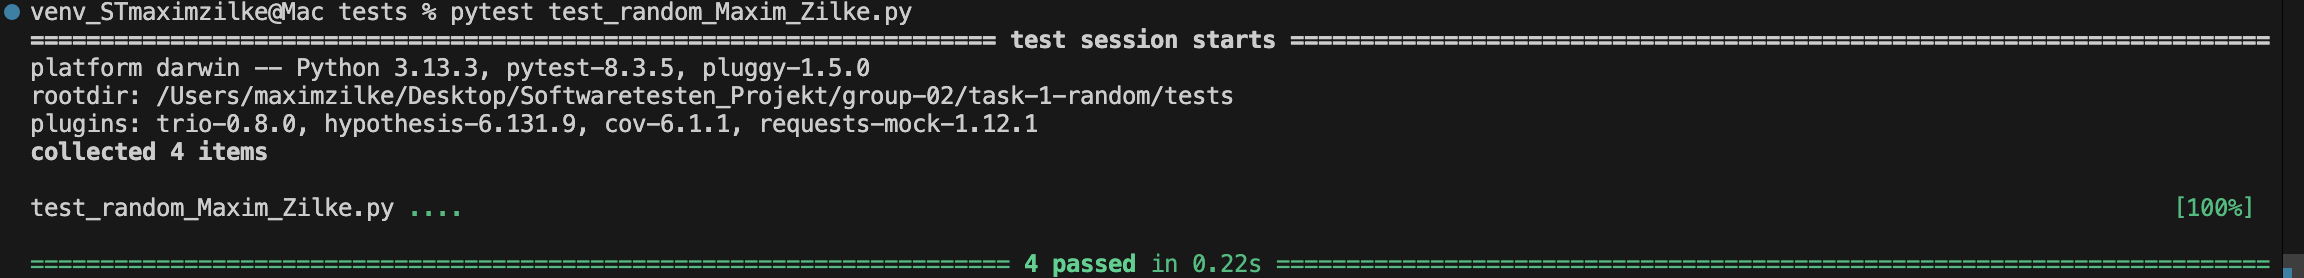
\includegraphics[width=1\textwidth]{test_isp_Maxim_Zilke.png} 
                \caption{Maxim Zilke – Random Test}
                \label{fig:maxim-random-test}
            \end{figure}
        [Yossef Al Buni] \\
    \begin{figure}[H]
        \centering
        \includegraphics[width=1\textwidth]{random\_testing\_Yossef\_AlBuni.png} 
        \caption{Yossef Al Buni – Random Test}
        \label{fig:maxim-random-test}
    \end{figure}
    \textbf{Test Execution:} In the terminal, the test file \texttt{test\_encrypt\_data\_4.py} was executed using the command \texttt{pytest test\_encrypt\_data\_4.py}. All 4 tests passed. \\
          \end{answer}
%%%%%%%%%%%%%%%%%%%%%%%%%%%%%%%%%%%%%%%%%%%%%%%%%%%%%%%%%%%%%%

% other members

%%%%%%%%%%%%%%%%%%%%%%%%%%%%%%%%%%%%%%%%%%%%%%%%%%%%%%%%%%%%%%
          
    \item Assess the input values generated by \texttt{hypothesis}. Do the tests represent meaningful scenarios?:
          \begin{answer}
        
%%%%%%%%%%%%%%%%%%%%%%%%%%%%%%%%%%%%%%%%%%%%%%%%%%%%%%%%%%%%%%
\begin{table}[ht]
\centering
\begin{tabular}{|l|l|}
\hline
\textbf{Prefix} & \textbf{Suffix} \\
\hline
jceqjupzs & pfyr \\
jceqjupzs & hdyajjnxvosy \\
jceqjupzs & jceqjupzs \\
\_bpzojxba & lgrl \\
\_bpzojxba & \_bpzojxba \\
 & akvgg \\
\_\_main\_\_ & q \\
\_\_main\_\_ & \_\_main\_\_ \\
true & heqj \\
heqj & heqj \\
vxgyia &  \\
wq & gwweugd \\
gwweugd & gwweugd \\
btoze &  \\
\hline
\end{tabular}
\caption{Beispielhafte Eingaben, generiert durch \texttt{hypothesis}}
\label{tab:hypothesis-inputs}
\end{table}
We wrote the test above for the \texttt{\_normalize\_key} function,  which replaces underscores (\texttt{\_}) in a string with hyphens (\texttt{-}). The Hypothesis test used randomly generated strings consisting of lowercase letters and underscores. For each test case, Hypothesis created two random string segments (\texttt{prefix} and \texttt{suffix}) and inserted an underscore between them to ensure at least one underscore was present. These inputs are partially meaningful. While some generated cases, such as \texttt{\_\_main\_\_}, resemble realistic configuration keys or environment variable names that might occur in practice, the majority of the inputs do not directly reflect typical real-world patterns. Most strings are random combinations of letters and underscores, which are unlikely to appear in actual usage contexts. Nevertheless, the test is still valuable, as it checks the correctness of the \texttt{\_normalize\_key} function across a wide range of possible inputs. It also validates the function's robustness when dealing with edge cases or malformed input. Although the generated data is not always realistic, the use of Hypothesis ensures extensive input space coverage, helping to reveal unexpected issues that might be missed with manually crafted test cases. Written by Maxim Zilke. \\
%%%%%%%%%%%%%%%%%%%%%%%%%%%%%%%%%%%%%%%%%%%%%%%%%%%%%%%%%%%%%%
\textbf{Yossef Al Buni} \\
    \begin{lstlisting}[caption={Yossef Al Buni -- Inputs for the Hypothesis-Tests in test\_encrypt\_data\_4}, label={lst:encryption}]
    === test_output_is_base64 ===
    Data: b'\xe6\xdff\xf7\xf2\xe1'
    Key: Xzj7QVcqFqKaG0AS8uQ8lVXrdRrKJ62
    IV : MqabCnlXQdLMEzfO
    
    === test_different_data_different_encryption ===
    Data1: b"\xc7\xc9\x8eh\xd6\xb7\xee\t\x80\x7f\xb33\xbed\xd1\xeb\xdc\xe0\x1fV\xd7\x1d/\x95\x01\xb4Q\n\xdf\x85\x04T\xc8\x87\xb45\x86'\xb4\xb7"
    Data2: b'\x8eg\x81\xd7\x18A9\xb8=&a\x1a@\xbd\x18\x8a\x9b\xac\xe8\xb3'
    Key  : AY2VXI83VfzeE2VkNkJU
    IV   : XNYda3Dj8qDJhUTg
    
    === test_deterministic_output ===
    Data: b'\x8a\xb1\x18x!\xe6\x15\xb6&'
    Key : U9UXI0UOSZ31bHoc86
    IV  : SmOfRigclNBTYiUE
    
    === test_output_not_empty ===
    Data: b'\xff'
    Key : 8di59auAp3LNhnF7j4lnc
    IV  : w8mbzDJAtfRlwbQB
    \end{lstlisting} 
\textbf{Answer to Question C:} Yes, the input values generated by Hypothesis represent meaningful and valid testing scenarios for the \texttt{encrypt\_data} method. Below, we provide an assessment of the test input values in each case to demonstrate their relevance and coverage. The examples used in the following tests are representative of realistic encryption use cases and effectively support the verification of the method’s expected behavior.

\textbf{Test 1: \texttt{test\_output\_is\_base64}}
\textbf{What is tested:}  
This test verifies that the output of the \texttt{encrypt\_data} function is valid Base64. If it were not, \texttt{base64.b64decode} would raise an error.
\textbf{Purpose:}  
The implementation explicitly encodes the result using \texttt{base64.b64encode()}, so we expect all outputs to be valid Base64. This test ensures that assumption holds for all valid inputs.
\textbf{Test 2: \texttt{test\_different\_data\_different\_encryption}}
\textbf{What is tested:}  
This test checks that encrypting different data with the same key and IV leads to different encrypted outputs.
\textbf{Purpose:}    
If different plaintexts produced the same ciphertext under AES-CBC, the encryption would be broken. This test confirms data sensitivity — a fundamental property of secure encryption.
\textbf*{Test 3: \texttt{test\_deterministic\_output}}
\textbf{What is tested:}  
This test ensures that the same input values always produce the same output.
\textbf{Purpose:}   
Deterministic behavior is expected for AES-CBC when key and IV are fixed. This test validates that no randomness or side effects affect the output.
\textbf{Test 4: \texttt{test\_output\_not\_empty}}
\textbf{What is tested:}  
This test asserts that the encrypted result is not an empty byte string.
\textbf{Purpose:}    
An empty output could indicate a failed encryption step. Ensuring a non-empty output is a basic sanity check for correct function behavior. \\
written by Yossef Al Buni. \\
%%%%%%%%%%%%%%%%%%%%%%%%%%%%%%%%%%%%%%%%%%%%%%%%%%%%%%%%%%%%%%

% other members

%%%%%%%%%%%%%%%%%%%%%%%%%%%%%%%%%%%%%%%%%%%%%%%%%%%%%%%%%%%%%%

          \end{answer}
  \end{enumerate}
\end{question}

\begin{aiTask}
  Assess the correctness and understandability of the LLM's generated tests applying the paper's methodology. Add any code relevant for your assessment to the answer:
  \begin{answer}
    [Group: Claude 4 Sonnet]

\section*{Prompt}
Hello, Claude. I am working on a project for my University. As a task, I am supposed to give you methods and you are supposed to write hypothesis tests for me. This is the original task: AI Review Task Recall RQ1: How understandable is the test suite provided by Chat- GPT? from the paper ChatGPT vs SBST: A Comparative Assessment of Unit Test Suite Generation covered in Research Task 02: • As a group, decide on methods of those selected above and instruct an LLM of arbi- trary choice to generate at least 4 tests using Hypothesis for random testing. • Assess the aspects of correctness and understandability of your own test cases in comparison to the LLM’s generated test cases according to the paper’s methodology described in its RQ1. • Document your selected LLM, your prompts, the generated test cases, and your assessment. My methods for you are the following: 


\begin{lstlisting}[language=Python]
@staticmethod
def _normalizekey(name: str) -> str:
    return name.replace("", "-")
\end{lstlisting}

Please write 4 tests for me. Important: Use Hypothesis



\section*{Correcness of test generateed by LLM}

To evaluate the effectiveness of the generated test cases by the LLM, we focus on the following three aspects from the paper \textit{ChatGPT vs SBST: A Comparative Assessment of Unit Test Suite Generation}:
(1) whether the LLM successfully produces a test case for each method under test;
(2) whether these test cases can be compiled and executed without errors; and
(3) whether the generated test cases are free from potential bugs or logical flaws.

Firstly, we were able to generate four test cases for our method with additional 4 test cases resulting in 8 overall, which fulfills the first criterion. After receiving the tests, we were able to use \texttt{pytest} to compile and run them without any errors. This shows that the tests generated works correctly, fulfilling the second criterion as well. For the last point, we do not have any additional software to test for bugs, but the tests appear to function as intended.

\begin{figure}[h]
    \centering
    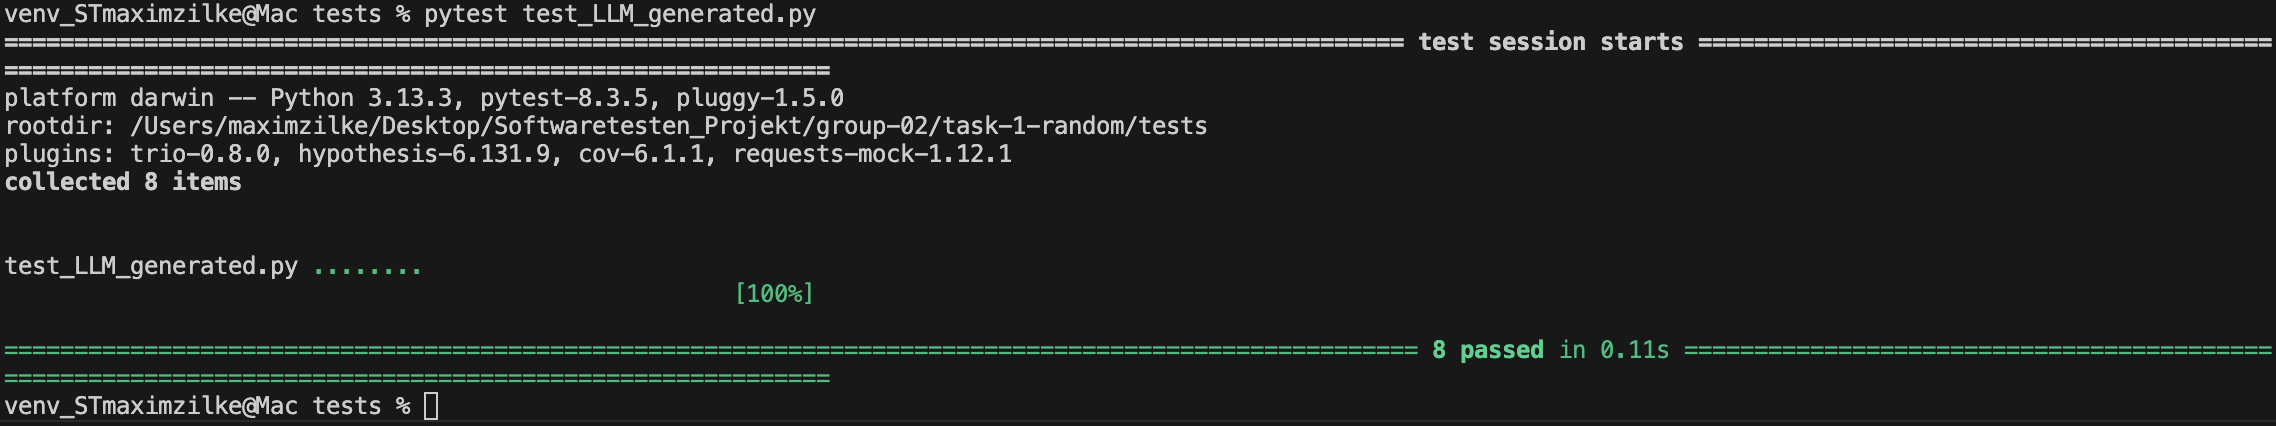
\includegraphics[width=1\textwidth]{LLM_Task_1.png} 
    \caption{Maxim Zilke Yossef Al Buni – Random Test}
    \label{fig:maxim-random-test}
\end{figure}

\section*{Comparison with Self-Written Tests}

If we now compare the actual content of the self-written and AI-generated tests, we find that the AI-generated tests cover a broader range of inputs, while the self-written test cases are more specific. Other than that, we would say that the AI and self-written tests assess the main functionality of the methods equally well. Additional we have four test cases which cover edge cases, this however was not asked for.


Written by Maxim Zilke and Yossef Al Buni
\section*{Tests}


\begin{lstlisting}[caption={Hypothesis-Test für \_normalize\_key by Maxim Zilke and Yossef Al Buni}, label={lst:normalize-key}]

import pytest
from hypothesis import given, strategies as st
import sys
from streamlink.options import Options


#class TestClass:
#    @staticmethod
#    def _normalize_key(name: str) -> str:
#        return name.replace("_", "-")


class TestNormalizeKey:
    
    @given(st.text())
    def test_normalize_key_returns_string(self, name):
        """Test that _normalize_key always returns a string regardless of input."""
        result = Options._normalize_key(name)
        assert isinstance(result, str)
    
    @given(st.text(alphabet=st.characters(blacklist_categories=('Cc', 'Cs'))))
    def test_normalize_key_no_underscores_in_output(self, name):
        """Test that the output never contains underscores."""
        result = Options._normalize_key(name)
        assert "_" not in result
    
    @given(st.text())
    def test_normalize_key_preserves_length_or_reduces(self, name):
        """Test that normalization doesn't increase string length."""
        result = Options._normalize_key(name)
        # Length should be preserved (underscores replaced 1:1 with hyphens)
        assert len(result) == len(name)
    
    @given(st.text(alphabet=st.characters(min_codepoint=32, max_codepoint=126)))
    def test_normalize_key_underscore_count_equals_hyphen_increase(self, name):
        """Test that the number of underscores in input equals the increase in hyphens in output."""
        original_hyphen_count = name.count("-")
        original_underscore_count = name.count("_")
        
        result = Options._normalize_key(name)
        result_hyphen_count = result.count("-")
        
        # The increase in hyphens should equal the original underscore count
        hyphen_increase = result_hyphen_count - original_hyphen_count
        assert hyphen_increase == original_underscore_count


# Additional specific test cases for edge cases
class TestNormalizeKeySpecific:
    
    def test_empty_string(self):
        """Test with empty string."""
        assert Options._normalize_key("") == ""
    
    def test_no_underscores(self):
        """Test string without underscores remains unchanged."""
        assert Options._normalize_key("hello-world") == "hello-world"
    
    def test_only_underscores(self):
        """Test string with only underscores."""
        assert Options._normalize_key("___") == "---"
    
    def test_mixed_underscores_and_hyphens(self):
        """Test string with both underscores and hyphens."""
        assert Options._normalize_key("hello_world-test_case") == "hello-world-test-case"

\end{lstlisting}




    
    % \begin{lstlisting}[style=pythongrey]
    % [LLM tests]
    % \end{lstlisting}
    % or: \lstinputlisting[style=pythongrey]{file_name.py}
  \end{answer}
\end{aiTask}

\end{document}
